\chapter{Geometry and Tracking MiceModule Properties}
In general, MAUS treats physical geometry distinct from fields. Fields can be placed overlapping physical
objects, or entirely independently of them, as the user desires. Properties for various aspects of the
physical and engineering model of the simulation are described below. This includes properties for
sensitive detectors.

\section{General Properties}
There are a number of properties that are applicable to any MiceModule.

\begin{center}
\tablefirsthead{\hline
{\bfseries Property} &
{\bfseries Type} &
{\bfseries Description}\\}
\tablehead{\hline
{\bfseries Property} &
{\bfseries Type} &
{\bfseries Description}\\}
\tabletail{}
\tablelasttail{}
\begin{supertabular}{|m{3.665cm}|m{1.278cm}|m{12.052cm}|}
\hline
Material &
string &
The material that the volume is made up from\\\hline
Invisible &
bool &
Set to 1 to make the object invisible in visualisation, or 0 to make the object visible.\\\hline
\multicolumn{2}{m{5.143cm}|}{\hspace*{-\tabcolsep}\begin{tabular}{|m{3.665cm}|m{1.278cm}}

RedColour &
double\\\hline
GreenColour &
double\\\hline
BlueColour &
double\\\hline
\end{tabular}\hspace*{-\tabcolsep}
} &
Alter the colour of objects as they are visualised\\\hhline{~~-}
G4StepMax &
double &
The maximum step length that Geant4 can make in the volume. Inherits values from the parent volumes.\\\hline
\multicolumn{2}{m{5.143cm}|}{\hspace*{-\tabcolsep}\begin{tabular}{|m{3.665cm}|m{1.278cm}}

G4TrackMax &
double\\\hline
G4TimeMax &
double\\\hline
\end{tabular}\hspace*{-\tabcolsep}
} &
The maximum track length and particle time of a track. Tracks outside this bound are killed. Inherits values from the
parent volumes.\\\hhline{~~-}
G4KinMin &
double &
The minimum kinetic energy of a track. Tracks outside this bound are killed. Inherits values from the parent
volumes.\\\hline
SensitiveDetector &
string &
Set to the type of sensitive detector required. Possible sensitive detectors are \textit{TOF}, \textit{SciFi},
\textit{CKOV}, \textit{SpecialVirtual, Virtual, Envelope} or \textit{EMCAL}.\\\hline
\end{supertabular}
\end{center}

\section{Sensitive Detectors}
A sensitive detector (one in which hits are recorded) can be defined by including the SensitiveDetector property. When a
volume is set to be a sensitive detector MAUS will automatically record tracks entering, exiting and crossing the
volume. Details such as the energy deposited by the track are sometimes also recorded in order to enable subsequent
modelling of the detector response.

Some sensitive detectors use extra properties.

\subsection[Scintillating Fibre Detector (SciFi)]{Scintillating Fibre Detector (SciFi)}
\subsection{Cerenkov Detector (CKOV)}
\subsection{Time Of Flight Counter (TOF)}
\subsection{Special Virtual Detectors}
Special virtual detectors are used to monitor tracking through a particular physical volume. Normally particle tracks
are written in the global coordinate system, although an alternate coordinate system can be defined. Additional
properties can be used to parameterise special virtual detectors.

\begin{center}
\tablefirsthead{\hline
{\bfseries Property} &
{\bfseries Type} &
{\bfseries Description}\\}
\tablehead{\hline
{\bfseries Property} &
{\bfseries Type} &
{\bfseries Description}\\}
\tabletail{}
\tablelasttail{}
\begin{supertabular}{|m{3.665cm}|m{1.3579999cm}|m{11.973001cm}|}
\hline
\multicolumn{2}{m{5.223cm}|}{\hspace*{-\tabcolsep}\begin{tabular}{|m{3.665cm}|m{1.3579999cm}}

ZSegmentation &
int\\\hline
PhiSegmentation &
int\\\hline
RSegmentation &
int\\\hline
\end{tabular}\hspace*{-\tabcolsep}
} &
Set the number of segments in the detector in Z, R or f. Defaults to 1.\\\hhline{~~-}
\multicolumn{2}{m{5.223cm}|}{\hspace*{-\tabcolsep}\begin{tabular}{|m{3.665cm}|m{1.3579999cm}}

SteppingThrough &
bool\\\hline
SteppingInto &
bool\\\hline
SteppingOutOf &
bool\\\hline
SteppingAcross &
bool\\\hline
\end{tabular}\hspace*{-\tabcolsep}
} &
Set to true to record tracks stepping through, into, out of or across the volume. Defaults to true.\\\hhline{~~-}
Station &
int &
Define an integer that is written to the output file to identify the station. Defaults to a unique integer identifier
chosen by MAUS, which will be different each time the same Special Virtual is placed.\\\hline
LocalRefRotation &
Hep3

Vector &
If set, record hits relative to a reference rotation in the coordinate system of the SpecialVirtual detector.\\\hline
GlobalRefRotation &
Hep3

Vector &
If set, record hits relative to a reference rotation in the coordinate system of the Configuration.\\\hline
LocalRefPosition &
Hep3

Vector &
If set, record hits relative to a reference position in the coordinate system of the SpecialVirtual detector.\\\hline
GlobalRefPosition &
Hep3

Vector &
If set, record hits relative to a reference position in the coordinate system of the Configuration.\\\hline
\end{supertabular}
\end{center}
\subsection{Virtual Detectors}
Virtual detectors are used to extract all particle data at a particular plane, irrespective of geometry. Virtual
detectors do not need to have a physical volume. The \textit{plane} can be a plane in z, time, proper time, or a
physical plane with some arbitrary rotation and translation.

\begin{center}
\tablefirsthead{\hline
{\bfseries Property} &
{\bfseries Type} &
{\bfseries Description}\\}
\tablehead{\hline
{\bfseries Property} &
{\bfseries Type} &
{\bfseries Description}\\}
\tabletail{}
\tablelasttail{}
\begin{supertabular}{|m{3.665cm}|m{1.3579999cm}|m{11.973001cm}|}
\hline
{\itshape IndependentVariable} &
String &
\liststyleLiv
\begin{itemize}
\item If set to \textit{t}, particle data will be written for particles at the time defined by the \textit{PlaneTime}
property. 
\end{itemize}
\liststyleLv
\begin{itemize}
\item If set to \textit{tau},\textit{ }particle data will be written for particles at the proper time defined by the
PlaneTime property. 
\end{itemize}
\liststyleLvi
\begin{itemize}
\item If set to \textit{z}, particle data will be written for particles crossing the module's z-position. 
\end{itemize}
\liststyleLvii
\begin{itemize}
\item If set to \textit{u}, particle data will be written for particles crossing a plane extending in \textit{x} and
\textit{y}.
\end{itemize}
\\\hline
{\itshape PlaneTime} &
Double &
If \textit{IndependentVariable} is \textit{t }or \textit{tau,} particle data will be written out at this time. Mandatory
if \textit{IndependentVariable} is \textit{t} or \textit{tau}.\\\hline
RadialExtent &
Double &
If set, particles outside this radius in the plane of the detector will not be recorded by the Virtual detector.\\\hline
GlobalCoordinates &
Bool &
If set to 0, particle data is written in the coordinate system of the module. Otherwise particle data is written in
global coordinates.\\\hline
MultiplePasses &
String &
Set how the VirtualPlane handles particles that pass through more than once. If set to Ignore, particles will be ignored
on second and subsequent passes. If set to SameStation, particles will be registered with the same station number. If
set to NewStation, particles will be registered with a NewStation number given by the \textit{(total number of
stations) + (this plane's station number)}, i.e. a new station number appropriate for a ring geometry.\\\hline
AllowBackwards &
Bool &
Set to false to prevent backwards-going particles from being recorded. Default is true.\\\hline
\end{supertabular}
\end{center}

\subsection{Envelope Detectors}
Envelope detectors are a type of Virtual detector that take all of the properties listed under virtual detectors, above.
In addition, in the optics application they can be used to interact with the beam envelope in a special way. The
following properties can be defined for Envelope Detectors \textit{in addition to} the properties specified above for
virtual detectors.

The The EnvelopeOut properties are used to make output from the envelope for use in the Optics optimiser.

\begin{center}
\tablefirsthead{\hline
{\bfseries Property} &
{\bfseries Type} &
{\bfseries Description}\\}
\tablehead{\hline
{\bfseries Property} &
{\bfseries Type} &
{\bfseries Description}\\}
\tabletail{}
\tablelasttail{}
\begin{supertabular}{|m{3.665cm}|m{1.3579999cm}|m{11.973001cm}|}
\hline
{\itshape EnvelopeOut1\_Name} &
String &
Defines the variable name that can be used as an expression substitution at the end of each iteration, typically
substituted into the Score parameters in the optimiser (see optimiser, below).\\\hline
{\itshape EnvelopeOut1\_Type} &
String &
Defines the type of variable that will be calculated for the substitution. Options are

\liststyleLviii
\begin{itemize}
\item Mean
\item Covariance
\item Standard\_Deviation
\item Correlation
\item Bunch\_Parameter
\end{itemize}
\\\hline
{\itshape EnvelopeOut1\_Variable} &
String &
Defines the variable that will be calculated for the substitution. Options are for Bunch\_Parameter

\liststyleLix
\begin{itemize}
\item \begin{itemize}
\item {\itshape emit\_6d \textup{: 6d emittance}}
\item {\itshape emit\_4d:\textup{ 4d emittance (in x-y space)}}
\item {\itshape emit\_t:\textup{ 2d emittance (in time space)}}
\item {\itshape emit\_x:\textup{ 2d emittance (in x space)}}
\item {\itshape emit\_y:\textup{ 2d emittance (in y space)}}
\item {\itshape beta\_4d:\textup{ 4d transverse beta function}}
\item {\itshape beta\_t:\textup{ 2d longitudinal beta function}}
\item {\itshape beta\_x: \textup{2d beta function (in(x space)}}
\item {\itshape beta\_y: \textup{2d beta function (in y space)}}
\item {\itshape alpha\_4d:\textup{ 4d transverse alpha function}}
\item {\itshape alpha\_t:\textup{ 2d longitudinal alpha function}}
\item {\itshape alpha\_x: \textup{2d alpha function (in(x space)}}
\item {\itshape alpha\_y: \textup{2d alpha function (in y space)}}
\item {\itshape gamma\_4d:\textup{ 4d transverse gamma function}}
\item {\itshape gamma\_t:\textup{ 2d longitudinal gamma function}}
\item {\itshape gamma\_x: \textup{2d gamma function (in(x space)}}
\item {\itshape gamma\_y: \textup{2d gamma function (in y space)}}
\item {\itshape disp\_x:\textup{ x-dispersion}}
\item {\itshape disp\_y:\textup{ y-dispersion}}
\item {\itshape ltwiddle:\textup{ normalised angular momentum}}
\item {\itshape lkin:\textup{ standard angular momentum}}
\end{itemize}

\end{itemize}
For Mean, Standard\_Deviation, Covariance and Correlation, variables should be selected from the options

\liststyleLx
\begin{itemize}
\item \textit{x: x-}position
\item {\itshape y:y-position}
\item {\itshape t: \textup{time}}
\item {\itshape px:\textup{ x-momentum}}
\item {\itshape py:\textup{ y-momentum}}
\item {\itshape E:\textup{ energy}}
\end{itemize}
For Mean, a single variable should be selected and value corresponding to the reference trajectory will be returned.

For Standard\_Deviation, a single variable should be selected and the 1 sigma beam size will be returned.

For Covariance and Correlation, two variables should be selected separated by a comma.\\\hline
\end{supertabular}
\end{center}
\section{Unconventional Volumes}
It is possible to define a number of volumes that use properties rather than the Dimensions keyword to define the volume
size.

{\sffamily\bfseries
Volume Trapezoid}

Volume Trapezoid gives a trapezoid which is not necessarily isosceles. Its dimensions are given by:

\begin{center}
\tablefirsthead{\hline
{\bfseries Property} &
{\bfseries Type} &
{\bfseries Description}\\}
\tablehead{\hline
{\bfseries Property} &
{\bfseries Type} &
{\bfseries Description}\\}
\tabletail{}
\tablelasttail{}
\begin{supertabular}{|m{3.665cm}|m{1.278cm}|m{12.052cm}|}
\hline
TrapezoidWidthX1 &
Double &
Gives width1 in x\\\hline
TrapezoidWidthX2 &
Double &
Gives width2 in x\\\hline
TrapezoidWidthY1 &
Double &
Gives height1 in y\\\hline
TrapezoidWidthY2 &
Double &
Gives height2 in y\\\hline
TrapezoidLengthZ &
Double &
Gives length along z\\\hline
\end{supertabular}
\end{center}
\subsection{Trapezoid Volume}
A Trapezoid Volume is like a Wedge Volume (look visualization below) with the possibility to have
different values for x width and 2 (non-zero) values for y.

\subsection{Volume Wedge}
A wedge is a triangular prism as shown in the diagram. Here the blue line extends along the positive z-axis and the red
line extends along the x-axis.
\begin{figure}[!p]
\begin{center}
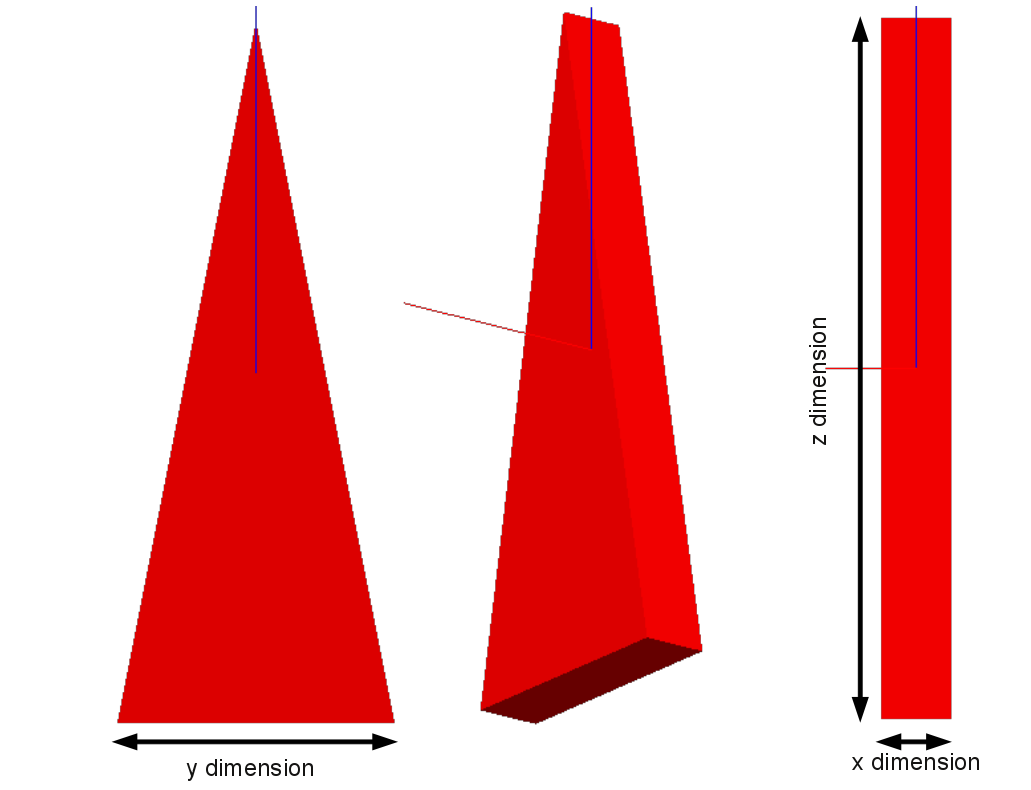
\includegraphics[width=13.968cm,height=8.394cm]{mice_modules/wedge_geometry.png}
\end{center}
\caption{Schematic of the geometry of a Wedge volume.}
\end{figure}
\begin{center}
\tablefirsthead{\hline
{\bfseries Property} &
{\bfseries Type} &
{\bfseries Description}\\}
\tablehead{\hline
{\bfseries Property} &
{\bfseries Type} &
{\bfseries Description}\\}
\tabletail{}
\tablelasttail{}
\begin{supertabular}{|m{3.665cm}|m{1.278cm}|m{12.052cm}|}
\hline
Dimensions &
Hep3

Vector &
\liststyleLxi
\begin{enumerate}
\item Width of the prism in x
\item Open end height of the prism in y
\item Length of the prism in z
\end{enumerate}
\\\hline
\end{supertabular}
\end{center}
\subsection{Volume Polycone}
A polycone is a volume of rotation, defined by a number of points in r and z. The volume is found by a linear
interpolation of the points.

\begin{center}
\tablefirsthead{\hline
{\bfseries Property} &
{\bfseries Type} &
{\bfseries Description}\\}
\tablehead{\hline
{\bfseries Property} &
{\bfseries Type} &
{\bfseries Description}\\}
\tabletail{}
\tablelasttail{}
\begin{supertabular}{|m{3.665cm}|m{1.278cm}|m{12.052cm}|}
\hline
PolyconeType &
string &
Set to Fill to define a solid volume of rotation. Set to Cone to define a shell volume of rotation with an inner and
outer surface.\\\hline
FieldMapMode &
string &
The name of the file that contains the polycone data.\\\hline
\end{supertabular}
\end{center}
\subsection{Volume Quadrupole}
Quadrupoles are defined by an empty cylinder with four further cylinders that are approximations to pole tips.

\begin{center}
\tablefirsthead{\hline
{\bfseries Property} &
{\bfseries Type} &
{\bfseries Description}\\}
\tablehead{\hline
{\bfseries Property} &
{\bfseries Type} &
{\bfseries Description}\\}
\tabletail{}
\tablelasttail{}
\begin{supertabular}{|m{3.665cm}|m{1.278cm}|m{12.052cm}|}
\hline
PhysicalLength &
double &
The length of the quadrupole container.\\\hline
QuadRadius &
double &
The distance from the quad centre to the outside of the quad.\\\hline
PoleTipRadius &
double &
The distance from the quad centre to the pole tip.\\\hline
CoilRadius &
double &
~
\\\hline
CoilHalfWidth &
double &
~
\\\hline
BeamlineMaterial &
string &
The material from which the beamline volume is made.\\\hline
QuadMaterial &
string &
The material from which the quadrupole volume is made.\\\hline
\end{supertabular}
\end{center}
\subsection{Volume Multipole}
Multipoles are defined by an empty box with an arbitrary number of cylinders that are approximations to pole tips. Poles
are placed around the centre of the box with n-fold symmetry. Multipoles can be curved, in which case poles cannot be
defined -- only a curved rectangular aperture will be present.

\begin{center}
\tablefirsthead{\hline
{\bfseries Property} &
{\bfseries Type} &
{\bfseries Description}\\}
\tablehead{\hline
{\bfseries Property} &
{\bfseries Type} &
{\bfseries Description}\\}
\tabletail{}
\tablelasttail{}
\begin{supertabular}{|m{3.892cm}|m{1.333cm}|m{11.77cm}|}
\hline
{\itshape ApertureCurvature} &
double &
Radius of curvature of the multipole aperture. For now curved apertures cannot have poles. Set to 0 for a straight
aperture.\\\hline
{\itshape ApertureLength} &
double &
Length of the multipole aperture.\\\hline
NumberOfPoles &
int &
Number of poles.\\\hline
PoleCentreRadius &
double &
The distance from the centre of the aperture to the centre of the cylindrical pole.\\\hline
PoleTipRadius &
double &
The distance from the centre of the aperture to the tip of the cylindrical pole.\\\hline
{\itshape ApertureInnerHeight} &
double &
The inner full height of the aperture.\\\hline
{\itshape ApertureInnerWidth} &
double &
The inner full width of the aperture.\\\hline
{\itshape AppertureOuterHeight} &
double &
The outer full height of the aperture.\\\hline
{\itshape ApertureOuterWidth} &
double &
The outer full width of the aperture.\\\hline
\end{supertabular}
\end{center}
\subsection{Volume Boolean}
Boolean volumes enable several volumes to be combined to make very sophisticated shapes from a number of elements.
Elements can be combined either by union, intersection or subtraction operations. A union creates a volume that is the
sum of two elements; an intersection creates a volume that covers the region where two volumes intersect each other;
and a subtraction creates a volume that contains all of one volume except the region that another volume sits in.

Boolean volumes combine volumes modelled by other MiceModules (submodules), controlled using the properties listed
below. Only the volume shape is used; position, rotation and field models etc are ignored. Materials, colours and other
relevant properties are all taken only from the Boolean Volume's properties.

Note that unlike in other parts of MAUS, submodules for use in Booleans (BaseModule, BooleanModule1, BooleanModule2
...) must be defined in a separate file, either defined in \$MICEFILES/Models/Modules or in the working directory.

Also note that visualisation of boolean volumes is rather unreliable. Unfortunately this is a feature of GEANT4. An
alternative technique is to use special virtual detectors to examine hits in boolean volumes.

\begin{center}
\tablefirsthead{\hline
{\bfseries Property} &
{\bfseries Type} &
{\bfseries Description}\\}
\tablehead{\hline
{\bfseries Property} &
{\bfseries Type} &
{\bfseries Description}\\}
\tabletail{}
\tablelasttail{}
\begin{supertabular}{|m{3.89cm}|m{1.333cm}|m{11.772cm}|}
\hline
{\itshape BaseModule} &
string &
Name of the physical volume that the BooleanVolume is based on. This volume will be placed at (0,0,0) with no rotation,
and all subsequent volumes will be added, subtracted or intersected with this one.\\\hline
{\itshape BooleanModule1} &
string &
The first module to add. MAUS will search for the MiceModule with path
\$MICEFILES/Models/Modules/{\textless}BooleanModule1{\textgreater}.\\\hline
{\itshape BooleanModule1Type} &
string &
The type of boolean operation to apply, either ``Union'', ``Intersection'' or ``Subtraction''.\\\hline
{\itshape BooleanModule1Pos} &
Hep3

Vector &
The position of the new volume with respect to the Base volume.\\\hline
{\itshape BooleanModule1Rot} &
Hep3

Vector &
The rotation of the new volume with respect to the Base volume.\\\hline
{\itshape BooleanModuleN} &
string &
Add extra modules as required. Replace ``N'' with the module number. N must be a continuous series incrementing by 1 for
each new module. Note that the order in which modules are added is important -- (A-B) \textsf{U }C is different to A-(B
\textsf{U }C).\\\hline
{\itshape BooleanModuleNType} &
\multicolumn{1}{m{1.333cm}}{string} &
\\\hhline{--~}
{\itshape BooleanModuleNPos} &
\multicolumn{1}{m{1.333cm}}{Hep3

Vector} &
\\\hhline{--~}
{\itshape BooleanModuleNRot} &
\multicolumn{1}{m{1.333cm}}{Hep3

Vector} &
\\\hhline{--~}
\end{supertabular}
\end{center}
\subsection{Volume Sphere}
A sphere is a spherical shell, with options for opening angles to make segments.

\begin{center}
\tablefirsthead{\hline
{\bfseries Property} &
{\bfseries Type} &
{\bfseries Description}\\}
\tablehead{\hline
{\bfseries Property} &
{\bfseries Type} &
{\bfseries Description}\\}
\tabletail{}
\tablelasttail{}
\begin{supertabular}{|m{3.89cm}|m{1.333cm}|m{11.772cm}|}
\hline
{\itshape Dimensions} &
Hep3

Vector &
The x value defines the inner radius. The y value defines the outer radius of the shell. The z value is not
used.\\\hline
Phi &
Hep3

Vector &
The x value defines the start opening angle in phi. The y value defines the end opening angle. The z value is not used.
Phi values must be in the range 0 to 360 degrees. If undefined, defaults to the range 0-360 degrees.\\\hline
Theta &
Hep3

Vector &
The x value defines the start opening angle in theta. The y value defines the end opening angle. The z value is not
used. Theta values must be in the range 0 to 180 degrees. If undefined, defaults to the range 0-360 degrees.\\\hline
\end{supertabular}
\end{center}

\section{Repeating Modules}
It is possible to set up a repeating structure for e.g. a repeating magnet lattice. The RepeatModule property enables
the user to specify that a particular module will be repeated a number of times, with all properties passed onto the
child module, but with a new position, orientation and scale factor. Each successive repetition will be given a
translation and a rotation relative to the coordinate system of the previous repetition, enabling the construction of
circular and straight accelerator lattices. Additionally, successive repetitions can have fields scaled relative to
previous repetitions, enabling for example alternating lattices.

\begin{center}
\tablefirsthead{\hline
{\bfseries Property} &
{\bfseries Type} &
{\bfseries Description}\\}
\tablehead{\hline
{\bfseries Property} &
{\bfseries Type} &
{\bfseries Description}\\}
\tabletail{}
\tablelasttail{}
\begin{supertabular}{|m{3.892cm}|m{1.333cm}|m{11.77cm}|}
\hline
{\itshape RepeatModule} &
bool &
Set to 1 to enable repeats in this module.\\\hline
{\itshape NumberOfRepeats} &
int &
Number of times the module will be repeated in addition to the initial placement.\\\hline
{\itshape RepeatTranslation} &
Hep3

Vector &
Translation applied to successive repeats, applied in the coordinate system of the previous repetition.\\\hline
{\itshape RepeatRotation} &
Hep3

Vector &
Rotation applied to successive repeats, applied in the coordinate system of the previous repetition.\\\hline
{\itshape RepeatScaleFactor} &
double &
ScaleFactor applied to successive repeats, applied relative to previous repetition's scale factor.\\\hline
\end{supertabular}
\end{center}
The RepeatModule2 property also enables the user to specify that a particular module will be repeated a number of times.
In this case, MAUS will set a substitution variable @RepeatNumber that holds an index between 0 and NumberOfRepeats.
This can be used in an expression in to provide a versatile interface between user and accelerator lattice.

\begin{center}
\tablefirsthead{\hline
{\bfseries Property} &
{\bfseries Type} &
{\bfseries Description}\\}
\tablehead{\hline
{\bfseries Property} &
{\bfseries Type} &
{\bfseries Description}\\}
\tabletail{}
\tablelasttail{}
\begin{supertabular}{|m{3.892cm}|m{1.333cm}|m{11.77cm}|}
\hline
{\itshape RepeatModule2} &
bool &
Set to 1 to enable repeats in this module.\\\hline
{\itshape NumberOfRepeats} &
int &
Number of times the module will be repeated in addition to the initial placement.\\\hline
\end{supertabular}
\end{center}

\section{Beam Definition and Beam Envelopes}
The Optics application can be used to track a trajectory and associated beam envelope through the accelerator structure.
Optics works by finding the Jacobian around some arbitrary trajectory using a numerical differentiation. This is used
to define a linear mapping about this trajectory, which can then be used to transport the beam envelope.

A beam envelope is defined by a reference trajectory and a beam ellipse. The reference trajectory takes its position and
direction from the position and rotation of the module. If no rotation is defined the reference trajectory is taken along
the z-axis. The magnitude of the momentum and the initial time of the reference trajectory is defined by properties. RF
cavities are phased using the reference trajectory defined here.

The beam ellipse is represented by a matrix, which can either be set using 

\begin{itemize}
\item Twiss-style parameters in $(x,px)$, $(y,py)$ and $(t,E)$ spaces.
\item Twiss-style parameters in $(t,E)$ space and Penn-style parameters in a cylindrically symmetric $(x,px,y,py)$ space.
\item A 6x6 beam ellipse matrix where the ellipse equation is given by $\mathbf{X}.\mathbf{T}() \mathbf{M} \mathbf{X} =
1$.
\end{itemize}
The Penn ellipse matrix is given by

\begin{equation*}
M=\left(\begin{matrix}\epsilon_Lmc\frac{\beta_L}{p}&-\epsilon_Lmc\alpha _L&0&0&0&0\\
       &\epsilon_Lmc\gamma_Lp&\frac{D_x}{E}V(E)&\frac{D_x'}{E}V(E)&\frac{D_y}{E}V(E)&\frac{D_y'}{E}V(E)\\
       &&\epsilon _Tmc\frac{\beta _T}{p}&-\epsilon_Tmc\alpha_T&0&-\epsilon _Tmc(\frac{q}{2}\beta _T\frac{B_z}{P}-L)\\
      &&&\epsilon _Tmc\gamma _Tp&\epsilon _Tmc(\frac{q}{
2}\beta _T\frac{B_z}{P}-L)&0\\&&&&\epsilon _Tmc\frac{\beta _T}{p}&-\epsilon _Tmc\alpha _T\\&&&&&\epsilon _Lmc\gamma
_Tp\end{matrix}\right)
\end{equation*}
Here $L$ is a normalised canonical angular momentum, $q$ is the reference particle charge,
$B_{z}$ is the nominal on-axis magnetic field, $p$ is the reference momentum,
$m$ is the reference mass, $\epsilon_T$ is the transverse emittance, $\beta_T$ and
$\alpha_{T}$ are the transverse Twiss-like functions, $\epsilon_{L}$ is the longitudinal emittance and
$\beta_{L}$ and $\alpha_{L}$ are the longitudinal Twiss-like functions. Additionally $D_{x}$,
$D_{y}$, $D'_{x}$ and $D'_{y}$ are the dispersions and their derivatives with respect to
$z$ and $V(E)$ is the variance of energy (given by the $(2,2)$ term in the matrix above).

The Twiss ellipse matrix is given by

\begin{equation*}
M=\left(\begin{matrix}\epsilon _Lmc\frac{\beta _L}{p}&-\epsilon _Lmc\alpha _L&0&0&0&0\\&\epsilon _Lmc\gamma
_Lp&\frac{D_x}{E}V(E)&\frac{D_x'}{E}V(E)&\frac{D_y}{E}V(E)&\frac{D_y'}{E}V(E)\\&&\epsilon _xmc\frac{\beta _x}{p}&-\epsilon
_xmc\alpha _x&0&0\\&&&\epsilon _xmc\gamma _xp&0&0\\&&&&\epsilon _ymc\frac{\beta _y}{p}&-\epsilon _ymc\alpha
_y\\&&&&&\epsilon _ymc\gamma _yp\end{matrix}\right)
\end{equation*}
Here \textit{p} is the reference momentum, \textit{m} is the reference mass, e\textsubscript{i}, b\textsubscript{i} and
a\textsubscript{i} are the emittances and Twiss functions in the (t,E), (x,p\textsubscript{x}) and
(y,p\textsubscript{y}) planes respectively, D\textsubscript{x}, D\textsubscript{y}, D'\textsubscript{x},
D'\textsubscript{y} are the dispersions and their derivatives with respect to z and V(E) is the variance of energy
(given by the (2,2) term in the matrix above).

\begin{center}
\tablefirsthead{\hline
{\bfseries Property} &
{\bfseries Type} &
{\bfseries Description}\\}
\tablehead{\hline
{\bfseries Property} &
{\bfseries Type} &
{\bfseries Description}\\}
\tabletail{}
\tablelasttail{}
\begin{supertabular}{|m{3.319cm}|m{1.2019999cm}|m{11.974cm}|}
\hline
{\itshape EnvelopeType} &
string &
Set to \textit{TrackingDerivative} to evolve a beam envelope in the Optics application.\\\hline
{\itshape BeamType} &
string &
Set to \textit{Random} to generate a beam using the parameters below for the Simulation application. Set to
\textit{Pencil }to generate a pencil beam (with no random distribution). Set to \textit{ICOOL}, \textit{Turtle,
MAUS\_PrimaryGenHit} or \textit{G4BeamLine} to use a beam file.\\\hline
{\itshape Pid} &
int &
The particle ID of particles in the envelope or beam.\\\hline
{\itshape Time} & double &
Set the time of the envelope reference trajectory\\\hline
{\itshape Longitudinal}
{\itshape Variable} &
string &
Set the longitudinal variable used to define the reference trajectory momentum. Options are \textit{Energy},
\textit{KineticEnergy, Momentum} and\textit{ ZMomentum.}\\\hline
\multicolumn{1}{m{3.319cm}}{\hspace*{-\tabcolsep}\begin{tabular}{|m{3.319cm}}

Energy\\\hline
KineticEnergy\\\hline
Momentum\\\hline
ZMomentum\\\hline
\end{tabular}\hspace*{-\tabcolsep}
} &
\hspace*{-\tabcolsep}\begin{tabular}{|m{1.2019999cm}}

double\\\hline
double\\\hline
double\\\hline
double\\\hline
\end{tabular}\hspace*{-\tabcolsep}
 &
Define the value of the longitudinal variable used to calculate the mean momentum and energy. The usual relationship
E\textsuperscript{2}+p\textsuperscript{2}c\textsuperscript{2}=m\textsuperscript{2}c\textsuperscript{4} applies. Kinetic
energy E\textsubscript{k} is related to energy E by E\textsubscript{k}+m=E.\\\hhline{~~-}
{\itshape EllipseDefinition} &
string &
Define the beam ellipse that will be used in calculating the evolution of the Envelope, or used to generate a beam for
BeamType \textit{Random}. Options are \textit{Twiss, Penn} and\textit{ Matrix}.\\\hline
\multicolumn{3}{|m{16.894999cm}|}{{\itshape The following properties are only used if EllipseDefinition is set to
Twiss}}\\\hline
\multicolumn{2}{m{4.721cm}|}{\hspace*{-\tabcolsep}\begin{tabular}{|m{3.319cm}|m{1.2019999cm}}

{\itshape Emittance\_X} &
double\\\hline
{\itshape Emittance\_Y} &
double\\\hline
{\itshape Emittance\_L} &
double\\\hline
\end{tabular}\hspace*{-\tabcolsep}
} &
Emittance in each 2d subspace, (x,px), (y,py) and (t,E).\\\hhline{~~-}
\multicolumn{2}{m{4.721cm}|}{\hspace*{-\tabcolsep}\begin{tabular}{|m{3.319cm}|m{1.2019999cm}}

{\itshape Beta\_X} &
double\\\hline
{\itshape Beta\_Y} &
double\\\hline
{\itshape Beta\_L} &
double\\\hline
\end{tabular}\hspace*{-\tabcolsep}
} &
Twiss b function in each 2d subspace, (x,px), (y,py) and (t,E).\\\hhline{~~-}
\multicolumn{2}{m{4.721cm}|}{\hspace*{-\tabcolsep}\begin{tabular}{|m{3.319cm}|m{1.2019999cm}}

{\itshape Alpha\_X} &
double\\\hline
{\itshape Alpha\_Y} &
double\\\hline
{\itshape Alpha\_L} &
double\\\hline
\end{tabular}\hspace*{-\tabcolsep}
} &
Twiss a function in each 2d subspace, (x,px), (y,py) and (t,E).\\\hhline{~~-}
\multicolumn{3}{|m{16.894999cm}|}{{\itshape The following properties are only used if EllipseDefinition is set to
Matrix}}\\\hline
\multicolumn{2}{m{4.721cm}|}{\hspace*{-\tabcolsep}\begin{tabular}{|m{3.319cm}|m{1.2019999cm}}

{\itshape Covariance(t,t)} &
double\\\hline
{\itshape Covariance(t,E)} &
double\\\hline
{\itshape Covariance(t,x)} &
double\\\hline
{\itshape ...} &
double\\\hline
{\itshape Covariance(Py,Py)} &
double\\\hline
\end{tabular}\hspace*{-\tabcolsep}
} &
Set the 6x6 matrix that will be used in the to define the beam ellipse. Covariances should be covariances of elements of
the matrix (x,Px,y,Py,t,E).

\ This must be a positive definite matrix, i.e. determinant {\textgreater} 0. Note that this means that at least the 6
terms on the diagonal must be defined. Other terms default to 0.\\\hline
\multicolumn{3}{|m{16.894999cm}|}{{\itshape The following properties are only used if EllipseDefinition is set to
Penn}}\\\hline
{\itshape Emittance\_T} &
double &
Transverse emittance for the 4d (x,px,y,py) subspace.\\\hline
{\itshape Emittance\_L} &
double &
Longitudinal emittance for the 2d (t,E) subspace.\\\hline
{\itshape Beta\_T} &
double &
Transverse beta for the 4d (x,px,y,py) subspace.\\\hline
{\itshape Beta\_L} &
double &
Longitudinal beta for the 2d (t,E) subspace.\\\hline
{\itshape Alpha\_T} &
double &
Transverse alpha for the 4d (x,px,y,py) subspace.\\\hline
{\itshape Alpha\_L} &
double &
Longitudinal alpha for the 2d (t,E) subspace.\\\hline
{\itshape Normalised}

{\itshape AngularMomentu} &
double &
Normalised angular momentum for the transverse phase space.\\\hline
Bz &
double &
Nominal magnetic field on the reference particle.\\\hline
\multicolumn{3}{|m{16.894999cm}|}{{\itshape The following properties are used if EllipseDefinition is set to Penn or
Twiss}}\\\hline
Dispersion\_X &
double &
Dispersion in x (x-energy correlation).\\\hline
Dispersion\_Y &
double &
Dispersion in y (y-energy correlation).\\\hline
DispersionPrime\_X &
double &
D' in x (Px-energy correlation).\\\hline
DispersionPrime\_Y &
double &
D' in y (Py-energy correlation).\\\hline
\multicolumn{3}{|m{16.894999cm}|}{{\itshape The following properties are only relevant for generating a beam
envelope}}\\\hline
RootOutput &
string &
Output file name for writing output beam envelope in ROOT binary format.\\\hline
LongTextOutput &
string &
Output file name for writing output beam envelope in string format.\\\hline
ShortTextOutput &
string &
Output file name for writing output beam envelope in string format. This abbreviated output omits some of the fields
that are present in LongTextOutput files.\\\hline
BeamOutput &
string &
If a BeamType is defined, this property controls the file name to which beam data is written.\\\hline
Delta\_t &
double &
Offset in time used for calculating numerical derivatives. Default is 0.1 ns.\\\hline
Delta\_E &
double &
Offset in energy used for calculating numerical derivatives. Default is 1 MeV.\\\hline
Delta\_x &
double &
Offset in x position used for calculating numerical derivatives. Default is 1 mm.\\\hline
Delta\_Px &
double &
Offset in x momentum used for calculating numerical derivatives. Default is 1 MeV/c.\\\hline
Delta\_y &
double &
Offset in y position used for calculating numerical derivatives. Default is 1 mm.\\\hline
Delta\_Py &
double &
Offset in y momentum used for calculating numerical derivatives. Default is 1 MeV/c.\\\hline
\multicolumn{2}{m{4.721cm}|}{\hspace*{-\tabcolsep}\begin{tabular}{|m{3.319cm}|m{1.2019999cm}}

Max\_Delta\_t &
double\\\hline
Max\_Delta\_E &
double\\\hline
Max\_Delta\_x &
double\\\hline
Max\_Delta\_Px &
double\\\hline
Max\_Delta\_y &
double\\\hline
Max\_Delta\_Py &
double\\\hline
\end{tabular}\hspace*{-\tabcolsep}
} &
Maximum offsets when polyfit algorithm is used. In some cases the offset can keep increasing without limit unless these
maximum offsets are defined. Default is no limit.\\\hhline{~~-}
\multicolumn{3}{|m{16.894999cm}|}{{\itshape The following properties are only relevant for generating a particle
beam}}\\\hline
UseAsReference &
Bool &
If set to true and the datacard \textit{FirstParticleIsReference} is set to 0, the first event in the Module will be
used as the reference particle that sets cavity phases. This particle will then have the mean trajectory (i.e. no
gaussian distribution).\\\hline
{\itshape BeamFile} &
string &
If the BeamType is \textit{ICOOL}, \textit{Turtle, MAUS\_PrimaryGenHit} or \textit{G4BeamLine}, this property defines
the name of the file containing tracks for MAUS.\\\hline
NumberOfEvents &
int &
Set the maximum number of events to take from this module. If other modules are defined, MAUS will iterate over the
modules until it the datacard \textit{numEvts} is reached or all modules have been run to \textit{NumberOfEvents}.
Default is for MAUS to keep tracking from the first module it finds until \textit{numEvts} is reached.\\\hline
\end{supertabular}
\end{center}
\section{Optimiser}
It is possible to define an optimiser for use in the Optics application. The optimiser enables the user to vary
parameters in the MiceModule file and try to find some optimum setting. For each value of the parameters, MAUS Optics
will calculate a score; the optimiser attempts to find a minimum value for this score.

\begin{center}
\tablefirsthead{\hline
{\bfseries Property} &
{\bfseries Type} &
{\bfseries Description}\\}
\tablehead{\hline
{\bfseries Property} &
{\bfseries Type} &
{\bfseries Description}\\}
\tabletail{}
\tablelasttail{}
\begin{supertabular}{|m{3.319cm}|m{1.2019999cm}|m{11.974cm}|}
\hline
{\itshape Optimiser} &
string &
Controls the function used for optimising. For now Minuit is the only available option.\\\hline
{\itshape Algorithm} &
string &
For \textit{Minuit} optimiser, controls the \textit{Minuit} algorithm used. In general Simplex is a good option to use
here. An alternative is Migrad. See Minuit documentation (for example at http://root.cern.ch/root/html/TMinuit.html)
for further information. Minuit attempts to minimise the score function defined by the Score properties.\\\hline
{\itshape NumberOfTries} &
int &
Maximum number of iterations MAUS will make in order to find the optimum value.\\\hline
{\itshape StartError} &
double &
Guess at the initial error in the score.\\\hline
{\itshape EndError} &
double &
Required final error in the score for the optimisation to converge successfully.\\\hline
RebuildSimulation &
bool &
Set to False to tell MAUS not to rebuild the simulation on each iteration. This should be used to speed up the
optimiser when a parameter is used that does not change the field maps. Default is true.\\\hline
{\itshape Parameter1\_Start} &
double &
Seed value for the parameter, that is used in the first iteration.\\\hline
{\itshape Parameter1\_Name} &
string &
Name of the parameter. This name is used as an expression substitution variable elsewhere in the code and should start
with @. See Expression Substitutions above for details on usage of expression substitutions.\\\hline
Parameter1\_Delta &
double &
Estimated initial error on the parameter. Default is 1.\\\hline
Parameter1\_Fixed &
bool &
Set to true to fix the parameter (so that it is excluded from the optimisation). Default is false.\\\hline
Parameter1\_Min &
double &
If required, set to the minimum value that the parameter can hold.\\\hline
Parameter1\_Max &
double &
If required, set to the maximum value that the parameter can hold.\\\hline

\multicolumn{2}{m{4.721cm}}{\hspace*{-\tabcolsep}\begin{tabular}{|m{3.319cm}|m{1.2019999cm}|}

Parameter2\_Start &
...\\\hline
... &
...\\\hline
Parameter2\_Max &
...\\\hline
{\itshape Score1} &
double\\\hline
Score2 &
...\\\hline
... &
...\\\hline
\end{tabular}\hspace*{-\tabcolsep}
} &
Define an arbitrary number of parameters. Parameters must be numbered consecutively, and each parameter must have at
least the start value and name defined. The optimiser will attempt to optimise against a score that is calculated by summing the Score1, Score2,... parameters
on each iteration.\\\hline
\end{supertabular}
\end{center}
